\documentclass[12pt]{report}
\usepackage[pdftex]{graphicx}
%\usepackage[pdftrex/bookmarksnumbered=true]{hyperref}
\usepackage{hyperref}
\linespread{1.5}
\textwidth = 6in
\textheight = 9in
\usepackage[body={6.0in, 8.2in},left=1.25in,right=1.0in,top=1.0in, bottom=1.0in]{geometry}
\frenchspacing
\usepackage{fancyhdr}
\usepackage{color}
\usepackage{xcolor}
\usepackage{listings}

\usepackage{caption}
\DeclareCaptionFont{white}{\color{white}}
\DeclareCaptionFormat{listing}{\colorbox{gray}{\parbox{\textwidth}{#1#2#3}}}
\captionsetup[lstlisting]{format=listing,labelfont=white,textfont=white}


\begin{document}
\pagenumbering{roman}
%\input{Coverpage.tex}

%----------------title page
\begin{titlepage}
\begin{center}
{\bf \large Decision Tree Classifier with GA based feature selection}\\
\vspace{.15in}
{\bfseries Mini Project Report}\\
\vspace{.15in}
{\normalsize Submitted to} \\
\vspace{.1in}
{\bfseries DEPARTMENT OF COMPUTER SCIENCE AND ENGINEERING}\\
\vspace{.25in}
{\normalsize \emph{By}}\\
{\bfseries\normalsize Samir Sheriff }\\
{\bfseries\normalsize Satvik N }\\
\vspace{.25in}
{\normalsize \emph{In partial fulfilment of the requirements\\ for the award of the degree \\
\vspace{.15in}
} } 

\vspace{.15in}
{\large{BACHELOR OF ENGINEERING}}\\
\vspace{.15in}
{\normalsize{IN}}\\
\vspace{.15in}
{\bfseries\normalsize COMPUTER SCIENCE AND ENGINEERING}\\
\vspace{0.15in}

\begin{figure}[h!]
	\centering
		\includegraphics[scale=0.5]{RVCE.png}
		
\end{figure} 
\vspace{.25in}
{\bfseries\large R V College of Engineering}\\
{\normalsize (Autonomous Institute, Affiliated to VTU)}\\
{\bfseries\normalsize BANGALORE - 560059}\\ 
{\bfseries\large May 2012}
\end{center}
\end{titlepage}


%---------Declaration
\begin{titlepage}
%\chapter*{\centerline{DECLARATION}}
\begin{center}
\section*{DECLARATION}
\end{center}

\paragraph{}  We, Samir Sheriff and Satvik N bearing USN number 1RV09CS093 and 1RV09CS095 respectively, hereby declare that the dissertation entitled ``\textbf{Decision Tree Classifier with GA feature selection}'' completed and written by us, has not been previously formed the basis for the award of any degree or diploma or certificate of any other University.
\vspace{1in}

\begin{flushright} {Bangalore \hspace{4.4in} Samir Sheriff } 
 {USN:1RV09CS093}
 \end{flushright}

\begin{flushright} { Satvik N } \\
 {USN:1RV09CS095}
 \end{flushright}
\end{titlepage}

%---------Certificate
\begin{titlepage}
\newpage
\begin{center}
{\bfseries\large R V COLLEGE OF ENGINEERING}\\
{\normalsize (Autonomous Institute Affiliated to VTU)}\\
{\normalsize DEPARTMENT OF COMPUTER SCIENCE AND ENGINEERING}\\
\end{center}
	
\begin{figure}[h!]
	\centering
		\includegraphics[scale=0.5]{RVCE.png}
		%\includegraphics{msrit-logo.jpg}
	%\caption{}
	%\label{fig:logo2}
\end{figure}

\begin{center}
\bf{\underline{CERTIFICATE}}
\end{center}
\noindent This is to certify that the dissertation entitled, ``\textbf{Decision Tree Classifier with GA based feature selection}'',  which is being submitted herewith for the award of B.E is the result of the work completed by \textbf{Samir Sheriff and Satvik N}  under my supervision and guidance.
\vspace{.5in}

\begin{flushleft} Signature of Guide 	
\\ (Name of the Guide) \\
\vspace{.5in}
 Signature of Head of Department  \hspace{4cm} Signature of Principal \\
 (Dr. N K Srinath) \hspace{6.6cm} (Dr. B.S Sathyanarayana)\\
 
 \end{flushleft} 
\begin{flushleft}
\hspace{1in}Name of Examiner \hspace{1.25in} Signature of Examiner
\end{flushleft}
\begin{flushleft}
1: \\
\vspace{.5in} 
2: 
\end{flushleft}
\end{titlepage}


%---------Acknowledgement
  
%\linespread{1.5}
\setcounter{page}{1}
\begin{center}
\section*{ACKNOWLEDGEMENT}
\addcontentsline{toc}{section}{ACKNOWLEDGEMENT}
\end{center}
The euphoria and satisfaction of the completion of the project will be incomplete
without thanking the persons responsible for this venture.


We acknowledge RVCE (Autonomous under VTU) for providing an opportunity to
create a mini-project in the 5th semester. We express our gratitude towards \textbf{Prof. B.S. Satyanarayana}, principal, R.V.C.E for constant encouragement and facilitates extended in completion of this project. We would like to thank \textbf{Prof. N.K.Srinath}, HOD, CSE
Dept. for providing excellent lab facilites for the completion of the project. We would
personally like to thank our project guides \textbf{Ms. Shantha Rangaswamy and Dr. } and also the lab in charge, for providing timely assistance \& guidance at the time.



We are indebted to the co-operation given by the lab administrators and lab assistants,
who have played a major role in bringing out the mini-project in the present form.
Bangalore



\begin{flushright}
Samir Sheriff\\
6th semester, CSE\\
USN:1RV09CS093\\

Satvik N\\
6th semester, CSE\\
USN:1RV09CS095\\

\end{flushright}

\newpage

%--------------Abstract
%\fontfamily{roman}%\selectfont
\begin{center}
\section*{ABSTRACT}
\addcontentsline{toc}{section}{ABSTRACT}
\end{center} 
Machine Learning techniques have been applied to the field of classification for more than a decade. Machine Learning techniques can learn normal and anomalous patterns from training data and generate classifiers, which
can be used to capture characteristics of interest. In general, the input data to classifiers is an extremely large set of features, but not all of features are relevant to the classes to be classified.
Hence, the learner must generalize from the given examples in order to produce a useful output in new cases. 

A major focus of machine learning research is the design of algorithms that recognize complex patterns and make intelligent decisions based on input data. Our Project, titled ``\textbf{Decision Tree Classifier with Genetic Algorithm-based Feature Selection}” is aimed at developing a complete program that constructs an optimal decision tree, based on any kind of data set, divided into training and testing examples, by selecting only a subset of features to classify data. 

Although our program works with generic data samples, it must be noted that when we started this project, our main intention was to classify ground water samples into two classes, namely Potable and Non-Potable Water. However, thanks to the miracle of Object-Oriented Programming Concepts, we were able to extend this project.



%------Table Of Contents
\addcontentsline{toc}{section}{CONTENTS}
\tableofcontents
%\listoffigures
%\listoftables


\newpage

\pagenumbering{arabic}
\setcounter{page}{1}

\pagestyle{fancy}
\lhead{\scriptsize{Introduction}}
\chead{}
\rhead{\scriptsize{Data Compression Techniques}}
\lfoot{\scriptsize{Dept. of CSE, R V C E, Bangalore.}}
\rfoot{\small{\thepage}}
\cfoot{\scriptsize{Feb 2012 - May 2013}}
\renewcommand{\headrulewidth}{0.4pt}
\renewcommand{\footrulewidth}{0.4pt}

\chapter{INTRODUCTION}


Machine learning, a branch of artificial intelligence, is about the construction and study of systems that can learn from data. The core of machine learning deals with representation and generalization. Representation of data instances and functions evaluated on these instances are part of all machine learning systems. There is a wide variety of machine learning tasks and successful applications. 






\section{SCOPE}

The machine learning concepts we have used in our project are listed below,
\begin{itemize}


\item{\textbf{Supervised learning}}  is the machine learning task of inferring a function from labeled training data. The training data consist of a set of training examples. In supervised learning, each example is a pair consisting of an input object (typically a vector) and a desired output value (also called the supervisory signal). A supervised learning algorithm analyzes the training data and produces an inferred function, which is called a classifier (if the output is discrete; see classification) or a regression function (if the output is continuous; see regression). The inferred function should predict the correct output value for any valid input object. This requires the learning algorithm to generalize from the training data to unseen situations in a "reasonable" way.

\item{\textbf{Decision tree learning}}, used in statistics, data mining and machine learning, uses a decision tree as a predictive model which maps observations about an item to conclusions about the item's target value. The goal is to create a model that predicts the value of a target variable based on several input variables.

\item A {\textbf{Genetic Algorithms}} is a search heuristic that mimics the process of natural evolution. This heuristic is routinely used to generate useful solutions to optimization and search problems. Genetic algorithms belong to the larger class of evolutionary algorithms (EA), which generate solutions to optimization problems using techniques inspired by natural evolution, such as inheritance, mutation, selection, and crossover.

\end{itemize}


\pagestyle{fancy}
\lhead{\scriptsize{Software Requirements Specification}}
\chead{}
\rhead{\scriptsize{Decision Tree Classifier with GA-based Feature Selection}}
\lfoot{\scriptsize{Dept. of CSE, R V C E, Bangalore.}}
\rfoot{\small{\thepage}}
\cfoot{\scriptsize{Feb 2012 - May 2013}}
\renewcommand{\headrulewidth}{0.4pt}
\renewcommand{\footrulewidth}{0.4pt}
\chapter{REQUIREMENT SPECIFICATION}
Software Requirement Specification (SRS) is an important part of the  software development process. We describe the overall description of the Mini-Project, the specific requirements of the Mini-Project, the software requirements and hardware requirements and the functionality of the system.



\subsubsection{Software Requirements}
\begin{itemize}

\item{	Front End: Java SWT Application.}
\item{	Back End: Java}
\item{	Operating System: Windows 7, Ubuntu 12.10.}

\end{itemize}

\subsubsection{Hardware Requirements}
\begin{itemize}
\item{Processor: Intel Core 2 Duo or higher version}
\item{RAM: 4GB or more}
\item{Hard disk: 5 GB or less}
\end{itemize}

%\input{IMP.tex}
\pagestyle{fancy}
\lhead{\scriptsize{Compression}}
\chead{}
\rhead{\scriptsize{Data Compression Techniques}}
\lfoot{\scriptsize{Dept. of CSE, R V C E, Bangalore.}}
\rfoot{\small{\thepage}}
\cfoot{\scriptsize{Feb 2012 - May 2013}}
\renewcommand{\headrulewidth}{0.4pt}
\renewcommand{\footrulewidth}{0.4pt}
\chapter{Decision Tree Learning}



\section{A Naive Approach}



\section{Definition}


Decision tree is the learning of decision tree from class labeled training tuples. A decision tree is a flow chart like structure, where each internal (non-leaf) node denotes a test on an attribute, each branch represents an outcome of the test, and each leaf (or terminal) node holds a class label. The topmost node in tree is the root node.

There are many specific decision-tree algorithms. Notable ones include:

\begin{itemize}
\item{\textbf{ID3} (Iterative Dichotomiser 3)}
\item{\textbf{C4.5} algorithm, successor of ID3}
\item{\textbf{CART} (Classification And Regression Tree)}
\item{\textbf{CHi-squared Automatic Interaction Detector }(CHAID). Performs multi-level splits when computing classification trees.}
\item{\textbf{MARS}: extends decision trees to better handle numerical data}
\end{itemize}


\section{The Basic Idea}

Decision tree is a classifier in the form of a tree structure (as shown in Fig. 3.1, where each node is either:
\begin{enumerate}
\item{A \textbf{leaf node} - indicates the value of the target attribute (class) of examples} (\textit{In Fig. 3.1, the nodes containing values K=x, K=y)}
\item{A \textbf{decision node} - specifies some test to be carried out on a single attribute-value, with one branch and sub-tree for each possible outcome of the test.\textit{In Fig. 3.1, the nodes containing attributes A, B and C)}}

\end{enumerate}

\begin{figure}[h!]
	\centering
		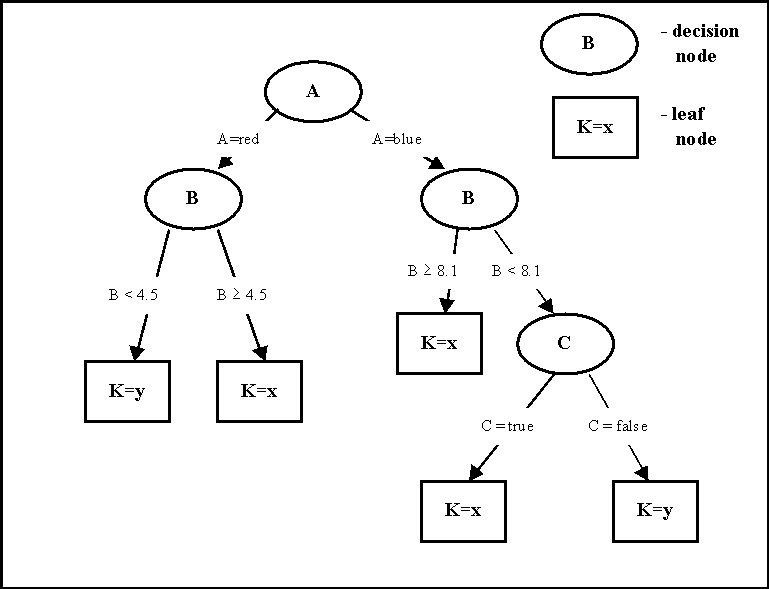
\includegraphics[scale=1.0]{dtreeexample.jpg}
	\caption{Sample Decision Tree}
	\label{fig:logo2}
\end{figure}

A decision tree can be used to classify an example by starting at the root of the tree and moving through it until a leaf node, which provides the classification of the instance.\\

Decision tree induction is a typical inductive approach to learn knowledge on classification. The key requirements to do mining with decision trees are:
\begin{itemize}
\item{\textbf{Attribute-value description}: object or case must be expressible in terms of a fixed collection of properties or attributes. This means that we need to discretize continuous attributes, or this must have been provided in the algorithm.\textit{(A, B and C, in Fig. 3.1)}}
\item{\textbf{Predefined classes (target attribute values)}: The categories to which examples are to be assigned must have been established beforehand (supervised data) \textit{(Classes X and Y in Fig. 3.1)}.}
\item{\textbf{Discrete classes}: A case does or does not belong to a particular class, and there must be more cases than classes.}
\item{\textbf{Sufficient data}: Usually hundreds or even thousands of training cases.}

\end{itemize}



\section{Building the Decision Tree}

Most algorithms that have been developed for learning decision trees are variations on a core algorithm that employs a top-down, greedy search through the space of possible decision trees. Decision tree programs construct a decision tree T from a set of training cases.


\subsection{ID3 Algorithm}
J. Ross Quinlan originally developed ID3 at the University of Sydney. He first presented ID3 in 1975 in a book, Machine Learning, vol. 1, no. 1. ID3 is based on the Concept Learning System (CLS) algorithm. ID3 searches through the attributes of the training instances and extracts the attribute that best separates the given examples. If the attribute perfectly classifies the training sets then ID3 stops; otherwise it recursively operates on the m (where m = number of possible values of an attribute) partitioned subsets to get their "best" attribute. The algorithm uses a greedy search, that is, it picks the best attribute and never looks back to reconsider earlier choices. Note that ID3 may misclassify data. 


\begin{figure}[h!]
	\centering
		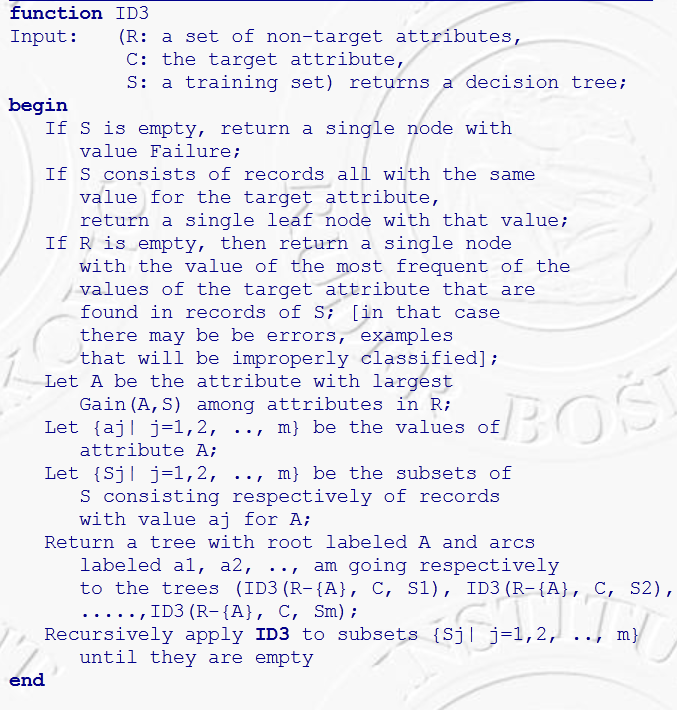
\includegraphics[scale=1.0]{ID3.png}
	\caption{ID3 Algorithm}
	\label{fig:ID3}
\end{figure}




\subsection{Choosing the best attribute for a given node}
The estimation criterion in the decision tree algorithm is the selection of an attribute to test at each decision node in the tree. The goal is to select the attribute that is most useful for classifying examples. A good quantitative measure of the worth of an attribute is a statistical property called information gain that measures how well a given attribute separates the training examples according to their target classification. This measure is used to select among the candidate attributes at each step while growing the tree. 

\subsection{Entropy - a measure of homogeneity of the set of examples}

In order to define information gain precisely, we need to define a measure commonly used in information theory, called entropy, that characterizes the (im)purity of an arbitrary collection of examples. Given a set S, containing only positive and negative examples of some target concept (a 2 class problem), the entropy of set S relative to this simple, binary classification is defined as:

\begin{math} Entropy(S) =  - p_{p}log_{2} p_{p} - p_{n}log_{2} p_{n} 
\end{math}

where p$_{p}$ is the proportion of positive examples in S and p$_{n}$ is the proportion of negative examples in S. In all calculations involving entropy we define 0 log 0 to be 0. 

To illustrate, suppose S is a collection of 25 examples, including 15 positive and 10 negative examples [15+, 10-]. Then the entropy of S relative to this classification is 

\begin{math} Entropy(S) = - (15/25) log_{2} (15/25) - (10/25) log_{2} (10/25) = 0.970 \end{math}


Notice that the entropy is 0 if all members of S belong to the same class. For example, if all members are positive (p$_{p}$= 1 ), then p$_{n}$ is 0, and:

\begin{math}Entropy(S) = -1 log_{2}(1) - 0 log_{2}0 = -1 0 - 0 log_{2}0 = 0. \end{math}

Note the entropy is 1 (at its maximum!) when the collection contains an equal number of positive and negative examples. If the collection contains unequal numbers of positive and negative examples, the entropy is between 0 and 1. Figure 3.3 shows the form of the entropy function relative to a binary classification, as p+ varies between 0 and 1. 


\begin{figure}[h!]
	\centering
		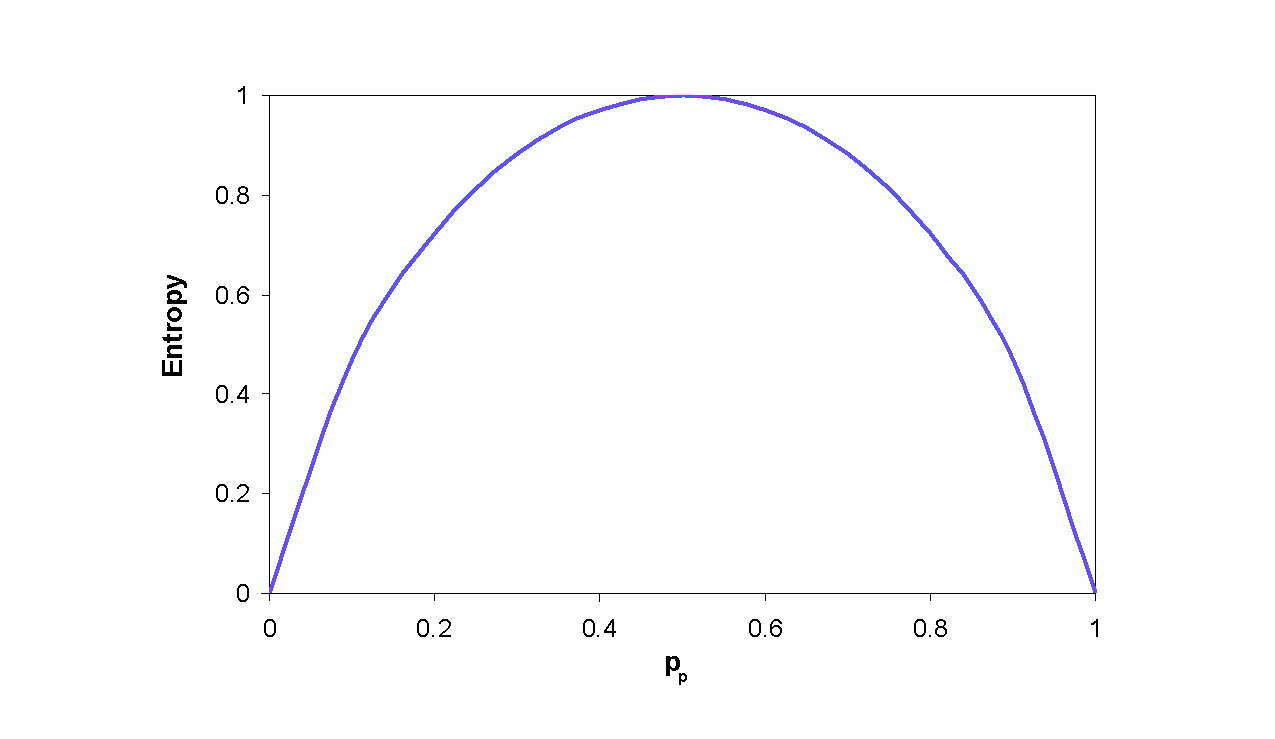
\includegraphics[scale=0.5]{entropy_graph.jpg}
	\caption{The entropy function relative to a binary classification, as the proportion of positive examples p$_{p}$ varies between 0 and 1.}
	\label{fig:ID3}
\end{figure}




One interpretation of entropy from information theory is that it specifies the minimum number of bits of information needed to encode the classification of an arbitrary member of S (i.e., a member of S drawn at random with uniform probability). For example, if p$_{p}$ is 1, the receiver knows the drawn example will be positive, so no message need be sent, and the entropy is 0. On the other hand, if p$_{p}$ is 0.5, one bit is required to indicate whether the drawn example is positive or negative. If p$_{p}$ is 0.8, then a collection of messages can be encoded using on average less than 1 bit per message by assigning shorter codes to collections of positive examples and longer codes to less likely negative examples.

Thus far we have discussed entropy in the special case where the target classification is binary. If the target attribute takes on c different values, then the entropy of S relative to this c-wise classification is defined as:

\begin{math}
Entropy(S) = \sum_{1}^{c} -p_{i} log_{2} p_{i}
\end{math}

where p$_{i}$ is the proportion of S belonging to class i. Note the logarithm is still base 2 because entropy is a measure of the expected encoding length measured in bits. Note also that if the target attribute can take on c possible values, the maximum possible entropy is log$_{2}$c. 

\subsection{Information gain measures the expected reduction in entropy}
Given entropy as a measure of the impurity in a collection of training examples, we can now define a measure of the effectiveness of an attribute in classifying the training data. The measure we will use, called information gain, is simply the expected reduction in entropy caused by partitioning the examples according to this attribute. More precisely, the information gain, Gain (S, A) of an attribute A, relative to a collection of examples S, is defined as:

\begin{math}
Gain(S, A) = Entropy(S) - \sum_{v \in Value(A)} \frac{S_{v}}{S} Entropy(S_{v})
\end{math}

where Values(A) is the set of all possible values for attribute A, and S$_{v}$ is the subset of S for which attribute A has value v (i.e., S$_{v}$ = {s Î S | A(s) = v}). Note the first term in the equation for Gain is just the entropy of the original collection S and the second term is the expected value of the entropy after S is partitioned using attribute A. The expected entropy described by this second term is simply the sum of the entropies of each subset S$_{v}$, weighted by the fraction of examples $|$S$_{v}$ $|$/$|S|$ that belong to S$_{v}$. Gain (S,A) is therefore the expected reduction in entropy caused by knowing the value of attribute A. Put another way, Gain(S,A) is the information provided about the target attribute value, given the value of some other attribute A. The value of Gain(S,A) is the number of bits saved when encoding the target value of an arbitrary member of S, by knowing the value of attribute A.

The process of selecting a new attribute and partitioning the training examples is now repeated for each non-terminal descendant node, this time using only the training examples associated with that node. Attributes that have been incorporated higher in the tree are excluded, so that any given attribute can appear at most once along any path through the tree. This process continues for each new leaf node until either of two conditions is met:

\begin{enumerate}
\item{Every attribute has already been included along this path through the tree}
\item{The training examples associated with this leaf node all have the same target attribute value (i.e., their entropy is zero).} 

\end{enumerate}


\section{An Example}

\subsection{An Example: "go go gophers"}


\subsection{Example Encoding Table}

The character encoding induced by the last tree is shown below where again, 0 is used for left edges and 1 for right edges.

\begin{figure}[h!]
	\centering
		%\includegraphics[scale=0.7]{huffTable1.png}
		%\includegraphics{msrit-logo.jpg}
	%\caption{}
	%\label{fig:logo2}
\end{figure}

\subsection{Encoded String}

The string "go go gophers" would be encoded as shown (with spaces used for easier reading, the spaces wouldn't appear in the real encoding).
\textbf{00 01 100 00 01 100 00 01 1110 1101 101 1111 1100}

Once again, 37 bits are used to encode "go go gophers". There are several trees that yield an optimal 37-bit encoding of "go go gophers". The tree that actually results from a programmed implementation of Huffman's algorithm will be the same each time the program is run for the same weights (assuming no randomness is used in creating the tree).



\pagestyle{fancy}
\lhead{\scriptsize{Decompression}}
\chead{}
\rhead{\scriptsize{Data Compression Techniques}}
\lfoot{\scriptsize{Dept. of CSE, R V C E, Bangalore.}}
\rfoot{\small{\thepage}}
\cfoot{\scriptsize{Feb 2012 - May 2013}}
\renewcommand{\headrulewidth}{0.4pt}
\renewcommand{\footrulewidth}{0.4pt}













\chapter{Genetic Algorithms}

Generally speaking, the process of decompression is simply a matter of translating the stream of prefix codes to individual byte values, usually by traversing the Huffman tree node by node as each bit is read from the input stream (reaching a leaf node necessarily terminates the search for that particular byte value). Before this can take place, however, the Huffman tree must be somehow reconstructed.

\section{Storing the Huffman Tree}

\begin{itemize}
\item In the simplest case, where character frequencies are fairly predictable, the tree can be preconstructed (and even statistically adjusted on each compression cycle) and thus reused every time, at the expense of at least some measure of compression efficiency.

\item Otherwise, the information to reconstruct the tree must be sent a priori.

\item A naive approach might be to prepend the frequency count of each character to the compression stream. Unfortunately, the overhead in such a case could amount to several kilobytes, so this method has little practical use.

\item Another method is to simply prepend the Huffman tree, bit by bit, to the output stream. For example, assuming that the value of 0 represents a parent node and 1 a leaf node, whenever the latter is encountered the tree building routine simply reads the next 8 bits to determine the character value of that particular leaf. The process continues recursively until the last leaf node is reached; at that point, the Huffman tree will thus be faithfully reconstructed. The overhead using such a method ranges from roughly 2 to 320 bytes (assuming an 8-bit alphabet). 

\begin{figure}[h!]
	\centering
		%\includegraphics[scale=0.7]{hufftreedecomp.png}
		%\includegraphics{msrit-logo.jpg}
	%\caption{}
	%\label{fig:logo2}
\end{figure}

\end{itemize}

Many other techniques are possible as well. In any case, since the compressed data can include unused "trailing bits" the decompressor must be able to determine when to stop producing output. This can be accomplished by either transmitting the length of the decompressed data along with the compression model or by defining a special code symbol to signify the end of input (the latter method can adversely affect code length optimality, however).


\section{Creating the Huffman Table}

To create a table or map of coded bit values for each character you'll need to traverse the Huffman tree (e.g., inorder, preorder, etc.) making an entry in the table each time you reach a leaf. For example, if you reach a leaf that stores the character 'C', following a path left-left-right-right-left, then an entry in the 'C'-th location of the map should be set to 00110. You'll need to make a decision about how to store the bit patterns in the map. At least two methods are possible for implementing what could be a class/struct BitPattern: 

\begin{itemize}

\item    Use a string. This makes it easy to add a character (using +) to a string during tree traversal and makes it possible to use string as BitPattern. Your program may be slow because appending characters to a string (in creating the bit pattern) and accessing characters in a string (in writing 0's or 1's when compressing) is slower than the next approach.

\item    Alternatively you can store an integer for the bitwise coding of a character. You need to store the length of the code too to differentiate between 01001 and 00101. However, using an int restricts root-to-leaf paths to be at most 32 edges long since an int holds 32 bits. In a pathological file, a Huffman tree could have a root-to-leaf path of over 100. Because of this problem, you should use strings to store paths rather than ints. A slow correct program is better than a fast incorrect program. 

\end{itemize}

\section{Storing Sizes}

The operating system will buffer output, i.e., output to disk actually occurs when some internal buffer is full. In particular, it is not possible to write just one single bit to a file, all output is actually done in "chunks", e.g., it might be done in eight-bit chunks. In any case, when you write 3 bits, then 2 bits, then 10 bits, all the bits are eventually written, but you can not be sure precisely when they're written during the execution of your program. Also, because of buffering, if all output is done in eight-bit chunks and your program writes exactly 61 bits explicitly, then 3 extra bits will be written so that the number of bits written is a multiple of eight. Because of the potential for the existence of these "extra" bits when reading one bit at a time, you cannot simply read bits until there are no more left since your program might then read the extra bits written due to buffering. This means that when reading a compressed file, you CANNOT use code like this.

\begin{verbatim}
	int bits; 
	while (input.readbits(1, bits)) 
	{ 
		// process bits 
	} 
\end{verbatim}



To avoid this problem, you can write the size of a data structure before writing the data structure to the file.
\pagestyle{fancy}
\lhead{\scriptsize{Conclusion}}
\chead{}
\rhead{\scriptsize{Data Compression Techniques}}
\lfoot{\scriptsize{Dept. of CSE, R V C E, Bangalore.}}
\rfoot{\small{\thepage}}
\cfoot{\scriptsize{Feb 2012 - May 2013}}
\renewcommand{\headrulewidth}{0.4pt}
\renewcommand{\footrulewidth}{0.4pt}
\chapter{CONCLUSION AND FUTURE WORKS}

\textbf{Summary}

\textbf{Limitations}
\begin{enumerate}
\item{Huffman code is optimal only if exact probability distribution of the source symbols is known.}
 
\item{Each symbol is encoded with integer number of bits.}
 
\item{Huffman coding is not efficient to adapt with the changing source statistics.}
 \item{The length of the codes of the least probable symbol could be very large to store into a single word or basic storage unit in a computing system.}
\end{enumerate}
	\textbf{Further enhancements}
The huffman coding the we have considered is simple binary Huffman codingbut many variations of Huffman coding exist,
\begin{enumerate}

\item{\textbf{ n-ary Huffman coding: }} The n-ary Huffman algorithm uses the \{0, 1, ... , n − 1\} alphabet to encode message and build an n-ary tree. This approach was considered by Huffman in his original paper. The same algorithm applies as for binary (n equals 2)codes, except that the n least probable symbols are taken together, instead of just the 2 least probable. Note that for n greater than 2, not all sets of source words can properly form an n-ary tree for Huffman coding. In this case, additional 0-probability place holders must be added. If the number of source words is congruent to 1 modulo n-1, then the set of source words will form a proper Huffman tree.
\item{\textbf{Adaptive Huffman coding: }}A variation called adaptive Huffman coding calculates the probabilities dynamically based on recent actual frequencies in the source string. This is some what related to the LZ family of algorithms.
\item{\textbf{Huffman template algorithm: }}Most often, the weights used in implementations of Huffman coding represent numeric probabilities, but the algorithm given above does not require this; it requires only a way to order weights and to add them. The Huffman template algorithm enables one to use any kind of weights (costs,frequencies etc)
\item{\textbf{Length-limited Huffman coding: }}Length-limited Huffman coding is a variant where the goal is still to achieve a minimum weighted path length, but there is an additional restriction that the length of each codeword must be less than a given constant. The package-merge algorithm solves this problem with a simple greedy approach very similar to that used by Huffman's algorithm. Its time complexity is O(nL),where L is the maximum length of a codeword. No algorithm is known to solve this problem in linear or linear logarithmic time, unlike the presorted and unsorted conventional Huffman problems, respectively.
%\item{\textbf{Huffman coding with unequal letter costs: }}Huffman coding with unequal letter costs is the generalization in which this assumption is no longer assumed true: the letters of the encoding alphabet may have non-uniform lengths, due to characteristics of the transmission medium. An example is the encoding alphabet of Morse code, where a 'dash' takes longer to send than a 'dot', and therefore the cost of a dash in transmission time is higher. The goal is still to minimize the weighted average codeword length,but it is no longer sufficient just to minimize the number of symbols used by the message. No algorithm is known to solve this in the same manner or with the same efficiency as conventional Huffman coding.Moreover we can extend the range of the huffman coding software to in corporate unicode which will require an interfacing module that will interpret a particular key in different languages based on the option selected. In that case the maximum number of symbols will be of the order of $2^{32}$
\end{enumerate}

\newpage

%For Bib refer to refs.bib to add/remove bib items
\addcontentsline{toc}{section}{BIBLIOGRAPHY}
\begin{thebibliography}{refs}
\bibitem{test}Genetic Algorithms  -\url{http://en.wikipedia.org/wiki/Genetic_algorithm}
\bibitem{t}Genetic Algorithm for constructing DT - \url{http://www.jprr.org/index.php/jprr/article/viewFile/44/25}
%\bibtitem{te}Decision Trees - \url{http://web.cecs.pdx.edu/~mm/MachineLearningWinter2010/pdfslides/DecisionTrees.pdf}
\bibitem{t} Project brief for the DT  using Horse data sets  - \url{https://cs.uwaterloo.ca/~ppoupart/teaching/cs486-spring06/assignments/asst4/asst4.pdf}
\bibitem{t}Supervised and Unsupervised Discretization of Continous Features - \url{http://robotics.stanford.edu/users/sahami/papers-dir/disc.pdf}
\bibitem{t}Hybrid learning using Genetic Algorithms and Decision Trees for pattern sification - \url{http://cs.gmu.edu/~eclab/papers/ijcai95.pdf}
\bibitem{t}Kardi Maams' Tutorials - \url{http://people.revoledu.com/kardi/tutorial/DecisionTree/index.html}

%\bibitem{}
%\bibitem{}
\end{thebibliography}

\newpage
\pagestyle{fancy}
\lhead{\scriptsize{Appendix A: Source Code}}
\chead{}
\rhead{\scriptsize{Data Compression Techniques}}
\lfoot{\scriptsize{Dept. of CSE, R V C E, Bangalore.}}
\rfoot{\small{\thepage}}
\cfoot{\scriptsize{Feb 2012 - May 2013}}
\renewcommand{\headrulewidth}{0.4pt}
\renewcommand{\footrulewidth}{0.4pt}

\addcontentsline{toc}{section*}{APPENDICES}
\section*{Appendices}
\section*{Appendix A : Source Code}
%\begin{lstinputlisting}[label=some-code,caption=Some Code]{Charnode.h}
%\lstinputlisting[ language=C++, label=charnode, caption=The definiton of the class Charnode\, each node of the huffman tree is an object of this class.]{Charnode.h}
%
%\lstinputlisting[language=C++, label=huffman,caption=The definition  of the class Huffman\, this class helps in building the huffman tree for an input file.]{HuffmanCode.h}
%
%\lstinputlisting[language=C++, label=compresswrite,caption=The definition  of the class CompressionWriting\, this class helps in writing the bits to the compressed file.]{CompressionWriting.h}
%
%\lstinputlisting[language=C++, label=huff,caption=The main program of the huffman compression algorithm.]{huff.cpp}
%
%\lstinputlisting[language=C++, label=unhuff,caption=The definition of the class Decompressor\, this class helps in decompressing the compressed file using huffman algorithm.]{Decompressor.h}
%
%\lstinputlisting[language=C++, label=unhuff,caption=The main program of the huffman decompression algorithm.]{unhuff.cpp}


%\lstinputlisting[language=C++, label=unhuff,caption=The definition of the class TCP\_Server\, an object of this class is a server object that can concurrently handle requests for files from the clients.]{TCP_Server.h}

%\lstinputlisting[language=C++, label=unhuff,caption=The definition of the class TCP\_Client\, an object of this class indicates a client object that can request for files from the server.]{TCP_Client.h}


\newpage
\pagestyle{fancy}
\lhead{\scriptsize{Appendix B: Screen shots}}
\chead{}
\rhead{\scriptsize{Decision Tree Classifier}}
\lfoot{\scriptsize{Dept. of CSE, R V C E, Bangalore.}}
\rfoot{\small{\thepage}}
\cfoot{\scriptsize{Sep 2012 - May 2013}}
\renewcommand{\headrulewidth}{0.4pt}
\renewcommand{\footrulewidth}{0.4pt}


\section*{Appendix B : Screen Shots}
\begin{figure}[h!]

  \centering
    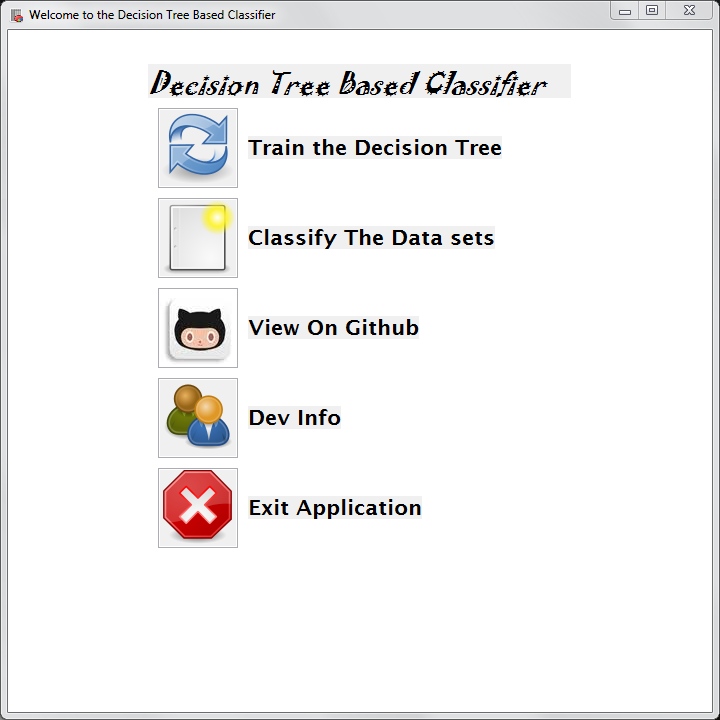
\includegraphics[scale=0.40]{welcome_window.png}
  \caption{Application Window - Welcome Screen}
\end{figure}

\begin{figure}[h!]
  
  \centering
    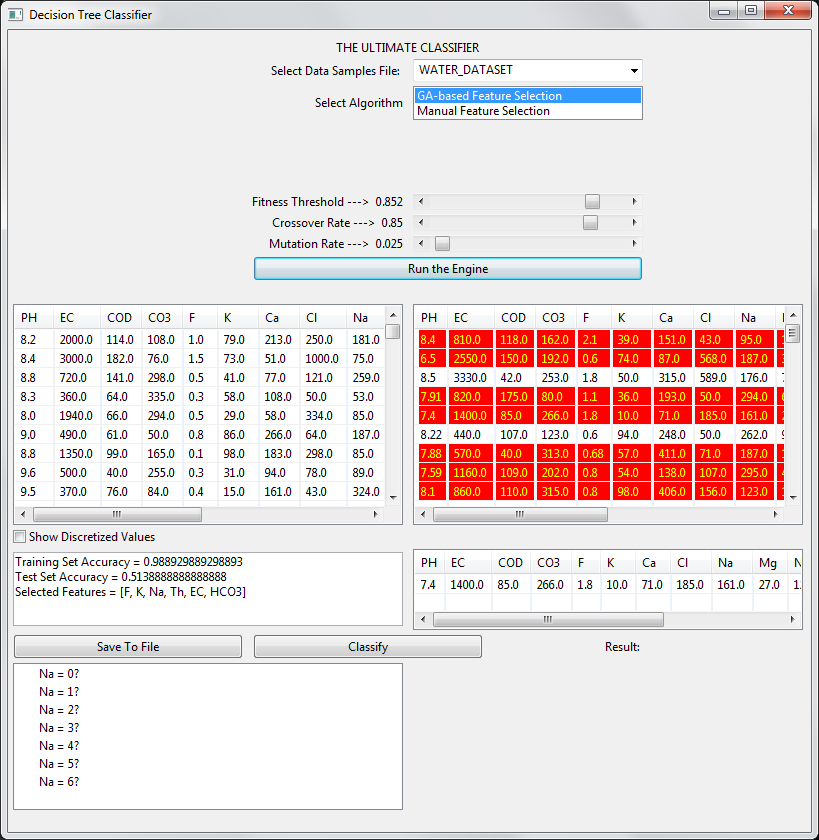
\includegraphics[scale=0.45]{dt_classifier.png}
\caption{Decision Tree Constructor Window.}
\end{figure}

\begin{figure}[h!]
  
  \centering
    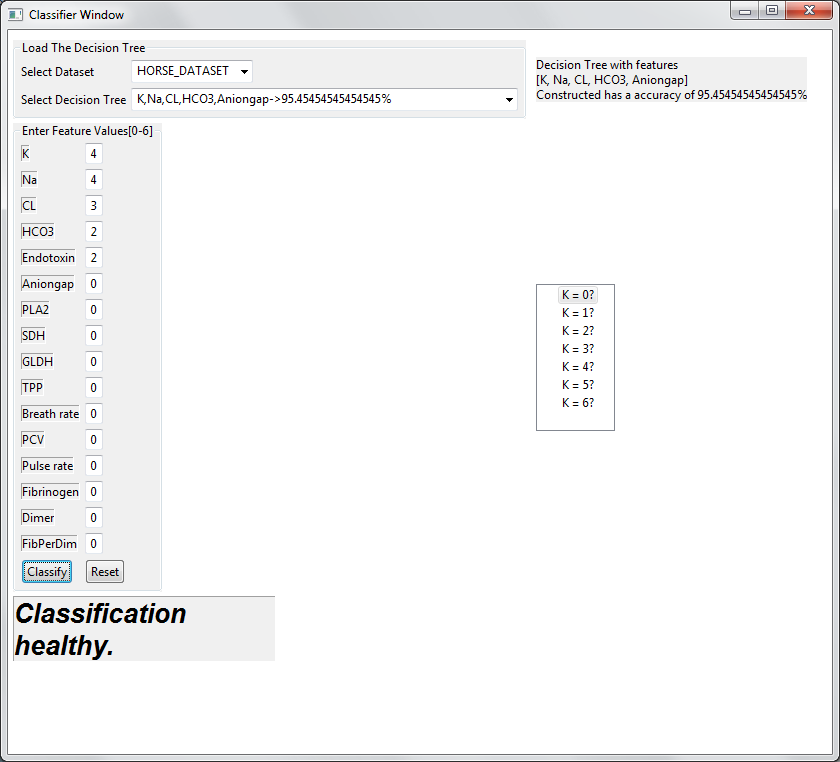
\includegraphics[scale=0.45]{dt_classification_window.png}
\caption{Decision Tree Classifier Window.}
\end{figure}
\begin{figure}[h!]
  
  \centering
    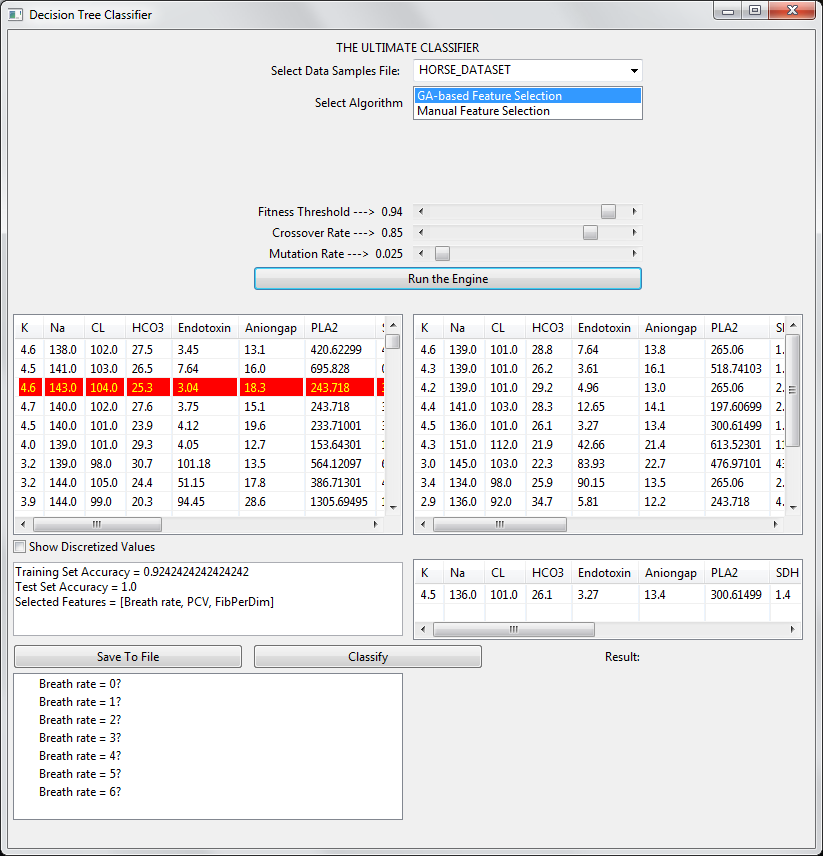
\includegraphics[scale=0.45]{dt_ga_algorithm.png}
\caption{Decision Tree Construction with GA based Feature Selector.}
\end{figure}

\begin{figure}[h!]
  
  \centering
    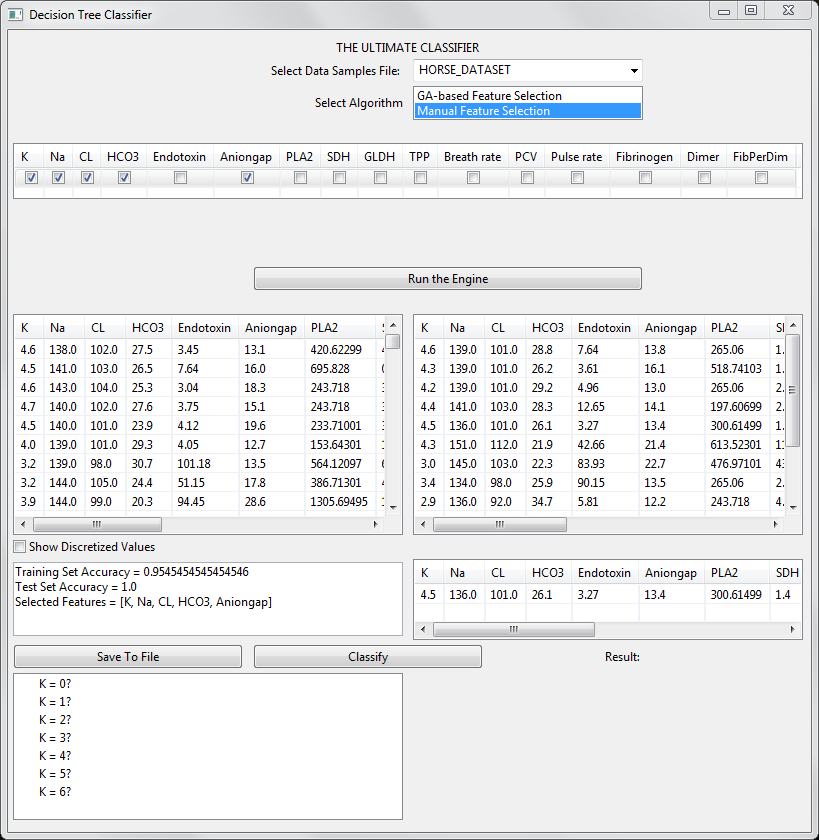
\includegraphics[scale=0.45]{dt_manual_selection.png}
\caption{Decision Tree Construction with manual feature selection.}
\end{figure}

\begin{figure}[h!]
  
  \centering
    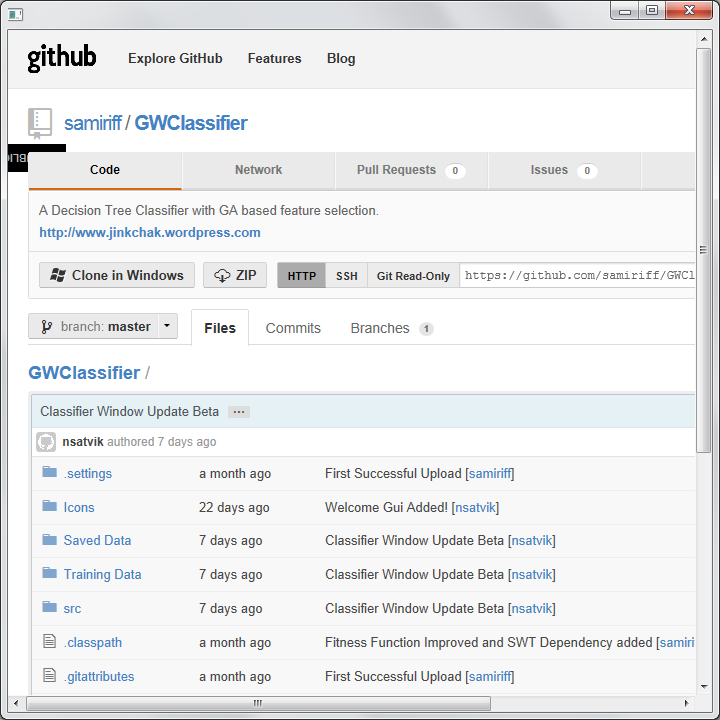
\includegraphics[scale=0.45]{git_hub.png}
\caption{The project source code on github public repository.}
\end{figure}


\end{document}
